\section{Primordial Magnetic Field Theory}

\subsection{Biermann Batteries}

The large-scale magnetic fields we see need to have had some initial seed field, but of course this raises the question: Where did the seed field come from? The most popular model for seed magnetic field generation from zero initial conditions is the Biermann battery \cite{Subramanian:2008tt}. Biermann batteries form in highly ionised environments such as the plasma shortly afer the Big Bang. Within the plasma, ions are drawn to regions of lower density and lower temperature. Since the the constituents of the plasma - protons and electrons - have different masses they flow at different rates resulting in a net flow of charge. If this flow of current forms a loop, then by Faraday's law of induction, a magnetic field is produced by the battery as shown in figure ~\ref{biermann}.

The magnetic field produced by the Biermann battery is described by:
\begin{equation}
\label{eqn:biermann}
\frac{\partial \vec{B}}{\partial t} = \nabla\times(\vec{U}\times\vec{B}-\eta\nabla \times\vec{B}) - \frac{c k_{b}}{e}\frac{\nabla n_e}{n_e} \times \nabla T
\end{equation}

The final term, $\nabla n_e \times \nabla T$ is the source term describing the Biermann battery effect. In order for this term to be non-zero and hence to have a Biermann battery, gradients of the electron density and the temperature must be non-parallel.

\begin{figure}[h]
\label{biermann}
\centering
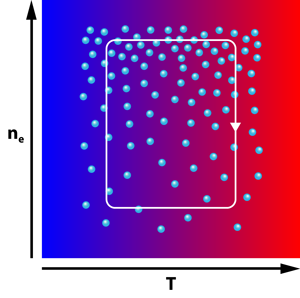
\includegraphics[scale=0.7]{images/biermann.png} 
\caption{The Biermann battery forms when the gradient between temperature and density are non-parallel. Ions move towards lower temperature and pressure zones. The difference in the mass of the positive and negative ions in the plasma leads to different flow rates, causing a net current. By Farday's law a magnetic field is produced by the Biermann battery. Figure from \cite{Biermann}}
\end{figure}

\subsection{Other Methods of PMF Generation}

\subsubsection{Inflation}
Cosmic inflation is an attactive model for PMF generation since it both explains how a seed magnetic field could end up coherent over megaparsec scales and provides a simple mechanism for generating a seed field from zero initial conditons. During inflation the seed field may emerge due to the absence of any ionised plasma during cosmic inflation. At this time the Universe isn't yet a good conductor. In this state the magnetic flux is not a conserved quantity and hence it is possible for a seed field to emerge spontaneously \cite{PhysRevD.37.2743}.

In inflationary theory, the exponential growth of the scale factor is responsible for stretching quantum fluctuations into large-scale density perturbations that seed large-scale structures such as galaxies and galaxy clusters. Similarly inflation may be able to take up a PMF field that spontaneously arises in the early Universe. A small scale fluctuation in the magnetic flux density could be stretched out over megaparsec scales and amplified by magnetohdydrodynamics in the intervening epochs between inflation and now \cite{PhysRevD.37.2743}.

A problem for this model is that it requires inflation to break conformal symmetry to produce this weak seed field initially. \cite{PhysRevD.37.2743} present one such model for conformal symmetry breaking leading to PMF generation as well as provide a deeper discussion of the reasons for studying inflation as the cause of PMF formation.
\\
\subsubsection{Phase Transitions}
PMFs may have also been produced by early phase transitions, such as the QCD transition or the electroweak phase transition. During a phase transition bubbles of the new phase form within the previous phase, these bubbles grow and collide until the entire Universe reaches the lower phase \cite{Yamazaki:2012pg}. These phase transitions induce  non-equilibrium processes such as leptogenesis and baryogenesis, which may be responsible for producing some weak magnetic fields. Within a phase transition, a collision between bubbles will produce turbulence leading to dynamos which will serve to spin up the magnetic fields into the strengths required to match the field strengths observed today.

\subsection{Galactic Dynamos as Amplifiers}
On their own, seed magnetic fields such as PMFs are too weak (of order nanoguass) to give rise to the magnetic fields we see in the cosmos today. There must be a process for amplifying the seed magnetic fields. Galactic dynamos are good candidates for seed magnetic field amplifiers \cite{beck}. Dynamos are systems that convert kinetic energy into electromagnetic energy. Hot ionised gas rotates around the galactic centre of a galaxy. The ions drag the magnetic field lines along with them, tangling them up and increasing the magnetic flux density, and in addition the magnetic field strength. Hence galactic dynamos are able to amplify a weak seed magnetic field into a stronger magnetic field that we observe today \cite{Subramanian:2008tt}.

\begin{figure}[ht]
\centering
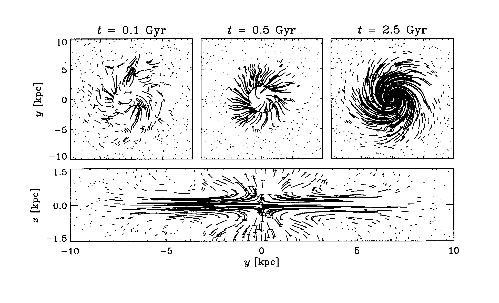
\includegraphics[scale=1]{images/dynamos_beck.png}
\caption{Spin up of magnetic fields in the presence of a galactic dynamo. In the first panel, at t = 0.1 Gyr, the seed magnetic field is picked up by a dynamo. Over the next two panels the dynamo spins up the magnetic field, increasing flux density. The bottom panel is a side-on view of the galactic dynamo at 8.1 Gyr. Figure from \cite{beck}.}
\end{figure}

\subsection{Effect of PMFs on the Cosmic Microwave Background}
If PMFs have a field strength of $\sim$1nG then their signatures will be detectable in the CMB B-mode polarisation power spectrum. Just as extragalactic magnetic fields Farday rotate radio and X-ray signals, PMFs would induce Faraday rotation within CMB polarisation. The net effect is that a fraction of E-mode polarisation would be transformed into B-mode polarisation. 
The PMF power spectrum is given by:

\begin{equation}
\label{eqn:pmfpower}
P(k) = A_{PMF}k^{n_{PMF}}
\end{equation}

Where $A_{PMF}$ is the PMF amplitude and $n_{PMF}$ is the PMF spectral index. Since the scale of the PMF power spectrum will depend on the age of the Universe when they first formed, the spectral index is sensitive to the mechanism that first produced PMFs.

\begin{figure}[h]
\label{fig:pmfpower}
\centering
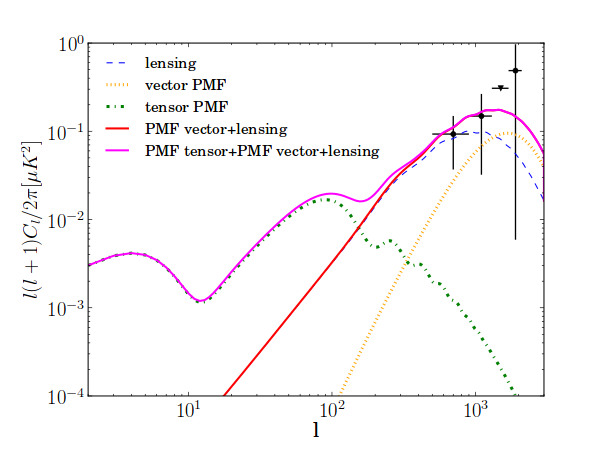
\includegraphics[scale=0.7]{images/PMFpower.png} 
\caption{Plot of the CMB power spectrum. The dotted green and yellow lines show the power spectrum for vector and tensor PMFs. Vector PMFs have more power on smaller scales (larger $\ell$) and tensor PMFs have more power on larger scales (smaller $\ell$). The purple line shows the expected combined PMF plus lensing effects on the CMB. Compared to the blue dotted line for lensing alone, a PMF-influenced CMB power spectrum may be detectable on smaller scales than on larger scales. Figure from \cite{Ade:2015cao}}
\end{figure}

In order to measure the strength of PMFs we focus our attention to the amplitude, $A_{PMF}$. The PMF amplitude is related to $B_{1Mpc}$, the strength of PMFs coherent over 1 megaparsec by the following relation:

\begin{equation}
\label{eqn:ab}
A_{PMF} = (\frac{B_{1Mpc}}{2.5nG})^4
\end{equation}

Recent work from Planck (2015) has constrained the primordial magnetic field strength coherent over 1 Mpc to $B_{1Mpc}$ $<$ 4.4nG \cite{Ade:2015cva}. In 2016 POLARBEAR modestly improved this constraint to $B_{1Mpc}$ $<$ 3.9nG \cite{Ade:2015cao}.
\subsection{Observable Effects of PMFs}

In addition to CMB polarisation, PMFs will affect large scale structure and Big Bang Nucleosynthesis (BBN).

\subsubsection{Large Scale Structure}

PMFs will indirectly shape the the structure of the cosmos. At early times a PMF can exert a Lorentz force on baryonic matter. Since baryonic matter interacts gravitationally with dark matter, it follows that PMFs have an influence on matter distribution. This effect can be observed in the density perturbation amplitude over 8 Mpc, $\sigma_8$ \cite{Yamazaki:2012pg}. One can also observe its effects by looking for changes in the matter power spectrum. Figure ~\ref{fig:matterpower} shows the impact of PMFs on the matter power spectrum for Universes with either massless or massive neutrinos.

\begin{figure}[ht]
\centering
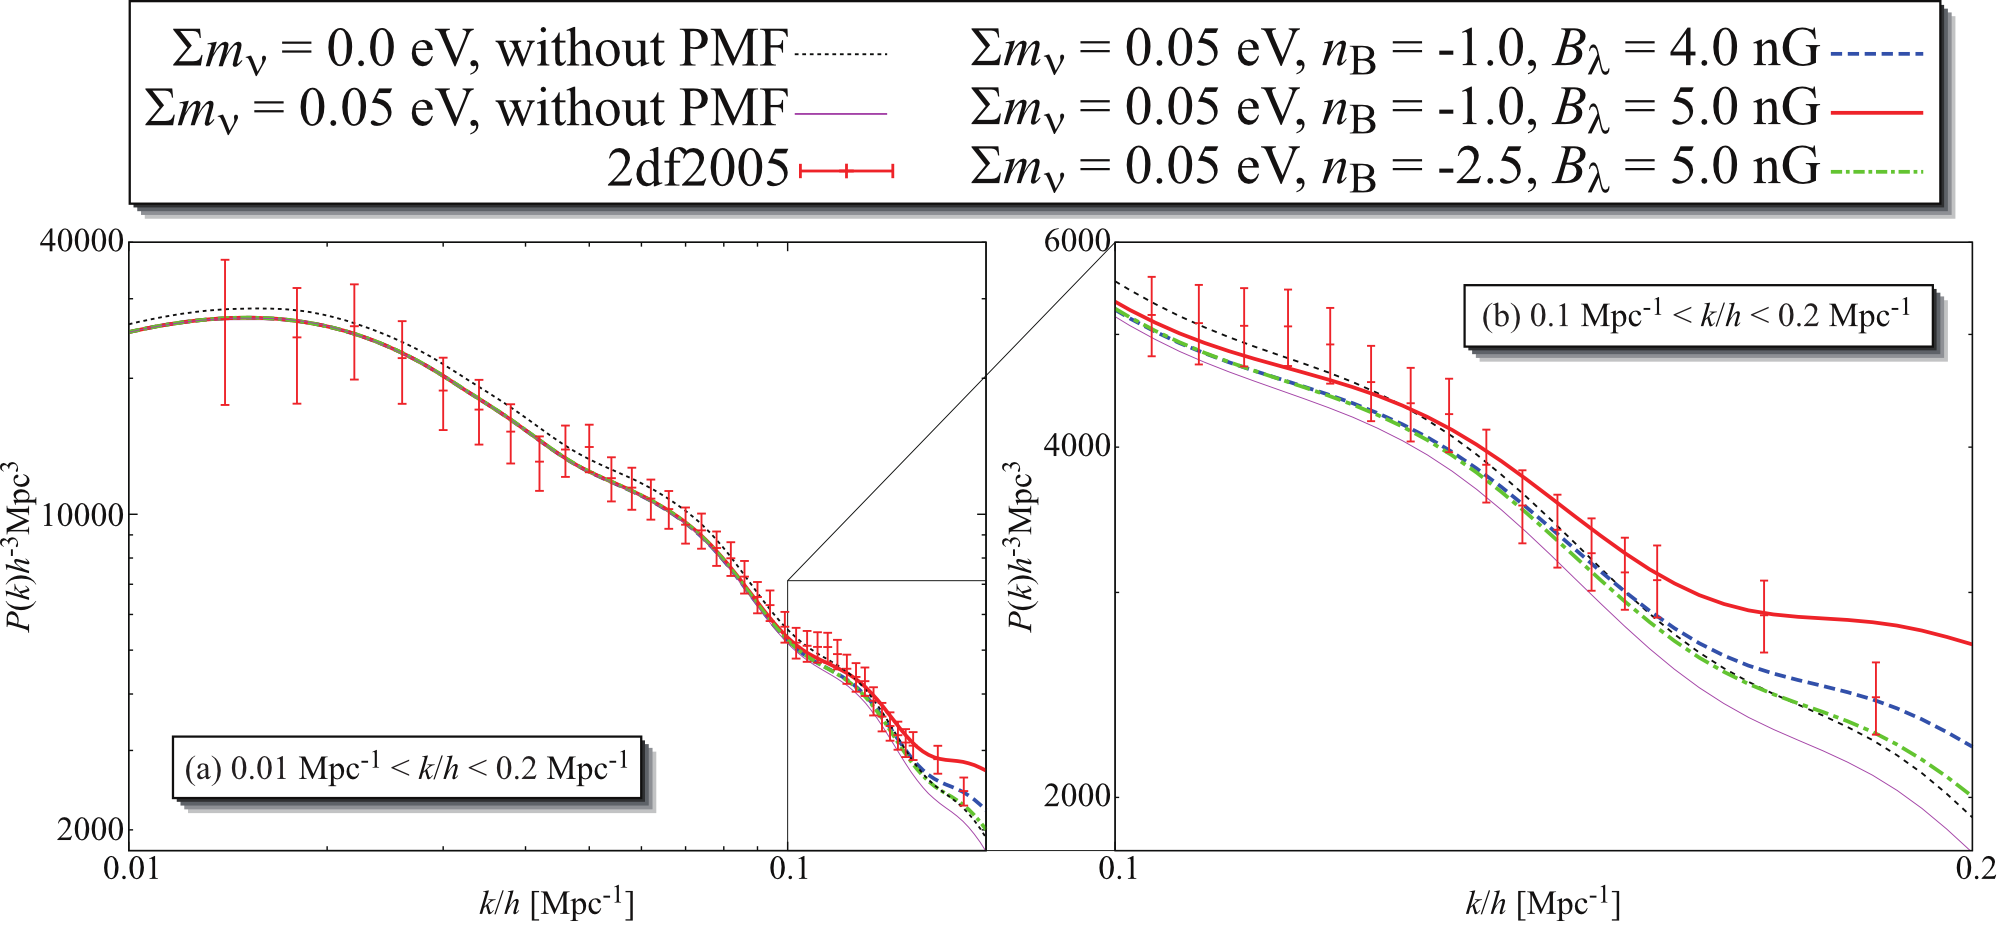
\includegraphics[scale=1.1]{images/matterpower.png} 
\caption{Plot of the matter power spectrum where k/h give the length scale. Here $B_{\lambda}$ is equal to $B_{1Mpc}$ The left panel gives the power spectrum in the range $0.01 Mpc^{-1} < k/h < 0.2 Mpc^{-1}$. At small scales (small k/h) all models fall within the experimental error, however the Universe without massive neutrinos or PMFs has more power at these scales. The right panel gives the power spectrum in the range $0.1 Mpc^{-1} < k/h < 0.2 Mpc^{-1}$. At larger scales, the matter power spectrum is significantly affected by the presence and strength of PMFs. Figure from \cite{Yamazaki:2012pg}}
\label{fig:matterpower}
\end{figure}

So far, there are no constraints on the PMF amplitude from large scale structure as the interactions happen in the non-linear regime, making predictions of its effects diffucult at the current time.


\subsubsection{Big Bang Nucleosynthesis}

If PMFs existed prior to BBN then we expect to see its signature in nuclear abundances \cite{PhysRevD.86.063003}. Primordial magnetic fields contribute to the overall energy density of the Universe and therefore vary the rate of expansion. If the rates of expansion in the Universe differ then so does the rate at which the Universe cools. If PMFs were indeed formed prior to BBN then the freeze-out times of reactions during BBN would differ from standard model values and hence so would primordial abundances of Helium and Hydrogen.

The strongest constraints from BBN have $B_{1Mpc}$ $<$ 1.5 $\mu G$ \cite{PhysRevD.86.063003}. These constraints are a thousand times weaker than those currently given by CMB polarisation measurements. We do not expect constraints from BBN to improve in the near future.

\subsection{Other Sources of Cosmic Birefringence}
Cosmic birefringence, which rotates E-mode polarisation to B-mode polarisation, is not a phenomenon unique to PMFs. Another mechanism for this effect may be quintessence. Quintessence is an alternative explanation to the cosmological constant for the accelerating expansion of the Universe. It argues that there may exist a long-range pseudoscalar field that can very weakly couple to baryons. The interaction is described by the Chern-Simmons term:
\begin{equation}
\label{eqn:chern}
\mathcal{L} \propto \frac{\phi}{2M}F_{\mu \nu}\tilde{F}^{\mu \nu}
\end{equation}

Where $\phi$ is the pseudoscalar field and M is the mass of the field boson. If photons couple to this field, then their polarisation will be rotated, just as they would if there were a PMF. The rotation angle due to the pseudoscalar field is given by:
\begin{equation}
\label{eqn:rotation}
\alpha = \frac{1}{M} \int{d\eta \dot{\phi}}
\end{equation}
Where $\dot{\phi}$ is integrated over the conformal time $\eta$

Currently we constrain the effects of cosmic birefringence with an equivalent effective PMF. Once we have made a detection, by comparing the two-point and four-point correlation functions it will be possible to differentiate between effects due to PMFs and effects due to conjectured quintessence models. \cite{Ade:2015cao}




